\documentclass{article}

\usepackage[margin=1in]{geometry}
\usepackage[utf8]{inputenc}
\usepackage{amsmath}
\usepackage{tikz}
\usepackage{sectsty}
\usetikzlibrary{automata,positioning}

\title{Homework \#2A}
\date{April 16th 2020}
\author{Zoe Sadeghi,\\University of Washington, Tacoma}

\sectionfont{\fontsize{12}{15}\selectfont}

\begin{document}

\maketitle

\section{Problem 1}

\paragraph{Part a}

\begin{center}
    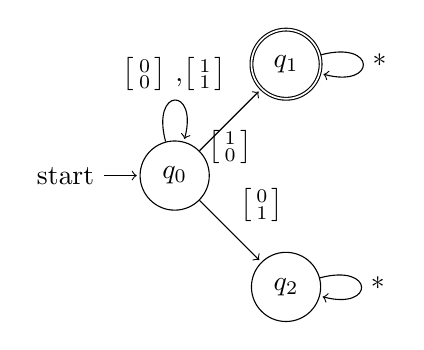
\begin{tikzpicture}[shorten >=1pt,node distance=2cm,on grid,auto] 
        \node[state,initial] (q_0)   {$q_0$}; 
        \node[state, accepting] (q_1) [above right=of q_0] {$q_1$}; 
        \node[state] (q_2) [below right=of q_0] {$q_2$}; 
        \path[->] 
        (q_0) edge node [anchor=north] {{$\bigl[ \begin{smallmatrix} 1\\ 0\end{smallmatrix}\bigr]$} } (q_1)
        (q_0) edge node {$\bigl[ \begin{smallmatrix} 0\\ 1\end{smallmatrix}\bigr]$} (q_2)
        (q_0) edge [loop above] node {{$\bigl[ \begin{smallmatrix} 0\\ 0\end{smallmatrix}\bigr]$} ,{$\bigl[ \begin{smallmatrix} 1\\ 1\end{smallmatrix}\bigr]$} }()
        (q_1) edge [loop right] node {*}()
        (q_2) edge [loop right] node {*}();
    \end{tikzpicture}
\end{center}

\begin{itemize}
    \item[$q_0$:] Most significant digit (MSD) is the same, so we can't accept or reject.
    \item[$q_1$:] We have already established that MSD for the top number is greater, the word is accepted.
    \item[$q_2$:] We have already established that MSD for the top number is smaller, the word is rejected.
\end{itemize}



\paragraph{Part b}

Let's start with the trivial case of the single letter word:

\begin{align*}
    &M_1 \subset M \land \forall m \in M_1 \ni |m| = 1 : M_1 = [1,0]
\end{align*}

We can see that our DFA only accepts $w=\bigl[\begin{smallmatrix}1\\0\end{smallmatrix}\bigr]$.

For the inductive step, we have the first case, which is composing $w_{n+1}$ with the assumption
that $w_n \in M$.

\begin{align*}
    W_n \in M &\Rightarrow r_i = q_1 \textrm{ (We must be in $q_1$ for $W_n$ to have been accepted)} \\
    & \Rightarrow \delta_(r_i, a) = q_1 \Rightarrow w_n+1 \in M 
\end{align*}

This correctly demontrates that concatenating anything to such a word would still result in an accepted word.

In the case where $w_n \notin M$, we should demontrate that resulting words are correct. In such a case, $w_n$
is unaccepted either because we were in $q_0$ or $q_2$. If we were in $q_0$, it is still possible to have a word
that is accepted, if we transition to $q_1$.

\begin{align*}
    &w_n \notin M \wedge \begin{cases}
        r_n = q_0 \wedge a = \bigl[\begin{smallmatrix}1\\0\end{smallmatrix}\bigr] & \delta(r_n,a)=q_1 \Rightarrow w_{n+q}\in M \\
        r_n = q_0 \wedge a \neq \bigl[\begin{smallmatrix}1\\0\end{smallmatrix}\bigr] & \delta(r_n,a) \in \{ q_0, q_2 \} \Rightarrow w_{n+q}\notin M \\
        r_n = q_2 & \delta(r_n,a) = q_2 \Rightarrow w_{n+q}\notin M
    \end{cases}
\end{align*}

\section{Problem 2}

\paragraph{Part a}

\begin{center}
    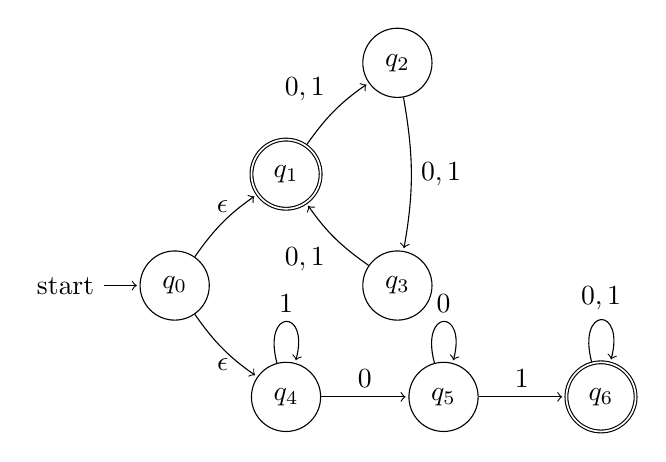
\begin{tikzpicture}[shorten >=1pt,node distance=2cm,on grid,auto] 
        \node[state,initial] (q_0)   {$q_0$}; 
        \node[state,accepting] (q_1) [above right=of q_0] {$q_1$}; 
        \node[state] (q_2) [above right=of q_1] {$q_2$}; 
        \node[state] (q_3) [below right=of q_1] {$q_3$}; 
        \node[state] (q_4) [below right=of q_0] {$q_4$}; 
        \node[state] (q_5) [right=of q_4] {$q_5$}; 
        \node[state,accepting] (q_6) [right=of q_5] {$q_6$}; 
        \path[->] 
        (q_0) edge [bend left=10] node [anchor=south] {$\epsilon$} (q_1)
              edge [bend right=10] node [anchor=north] {$\epsilon$} (q_4)
        (q_2) edge [bend left=10] node {$0,1$} (q_3)
        (q_1) edge [bend left=10] node {$0,1$} (q_2)
        (q_3) edge [bend left=10] node {$0,1$} (q_1)
        (q_4) edge [loop above] node {$1$} ()
              edge node {$0$} (q_5)
        (q_5) edge [loop above] node {$0$} ()
              edge node {$1$} (q_6)
        (q_6) edge [loop above] node {$0,1$} ();
    \end{tikzpicture}
\end{center}

\paragraph{Part b}

for any given NFA N, we will need a start state and then the NFA will need to transition to some accepting state on input 0. If this is the same state as the starting state of N, then $ L = {\epsilon , 0} $. Therefore, we will need a second state.

\section{Problem 3}

\paragraph{Part a}

\begin{center}
    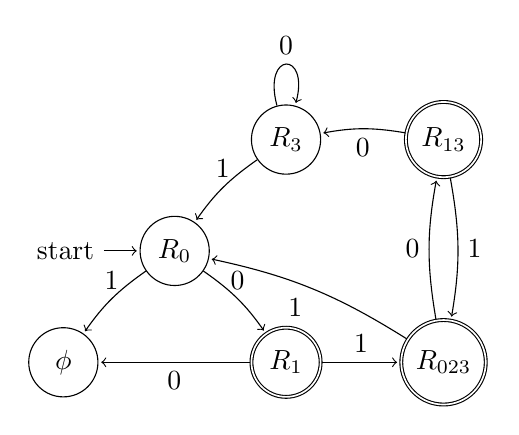
\begin{tikzpicture}[shorten >=1pt,node distance=2cm,on grid,auto] 
        \node[state,initial] (R_0)   {$R_0$}; 
        \node[state] (phi) [below left=of R_0] {$\phi$}; 
        \node[state,accepting] (R_1) [below right=of R_0] {$R_1$}; 
        \node[state,accepting] (R_023) [right=of R_1] {$R_{023}$}; 
        \node[state] (R_3) [above right=of R_0] {$R_3$}; 
        \node[state,accepting] (R_13) [right=of R_3] {$R_{13}$}; 
        \path[->] 
        (R_0) edge [bend right=10] node [anchor=south] {$1$} (phi)
              edge [bend left=10] node [anchor=south] {$0$} (R_1)
        (R_1) edge node {$0$} (phi)
              edge node {$1$} (R_023)
        (R_023) edge [bend right=10] node {$1$} (R_0)
                edge [bend left=10] node {$0$} (R_13)
        (R_3) edge [loop above] node {$0$} ()
              edge [bend right=10] node [anchor=south] {$1$} (R_0)
        (R_13) edge [bend left=10] node {$1$} (R_023)
               edge [bend right=10] node {$0$} (R_3);
    \end{tikzpicture}
\end{center}

\paragraph{Part b}

\begin{align*}
& M = (Q',\Sigma',\delta', q_0',F')\\
& Q' = P(Q)\\
& \Sigma' = \Sigma \\
& \delta'(R,a)=\{ q | q \in E(\bigcup\limits_{r \in R} \delta(r,a)) \} \\
& q_0'=\{ q_0 \} \\
& F' = \{ R | q_1 \in R \vee q_2 \in R \}
\end{align*}

where $P$ is the powerset generator function and $E$ is the $\epsilon$ transition superset.

\paragraph{Part c}
$ |P(Q)| = 2^{|Q|} = 2 ^ 4 = 16$

\paragraph{Part d}

The answer is 6.

\end{document}  

